\begin{figure}[H]
\begin{center}
    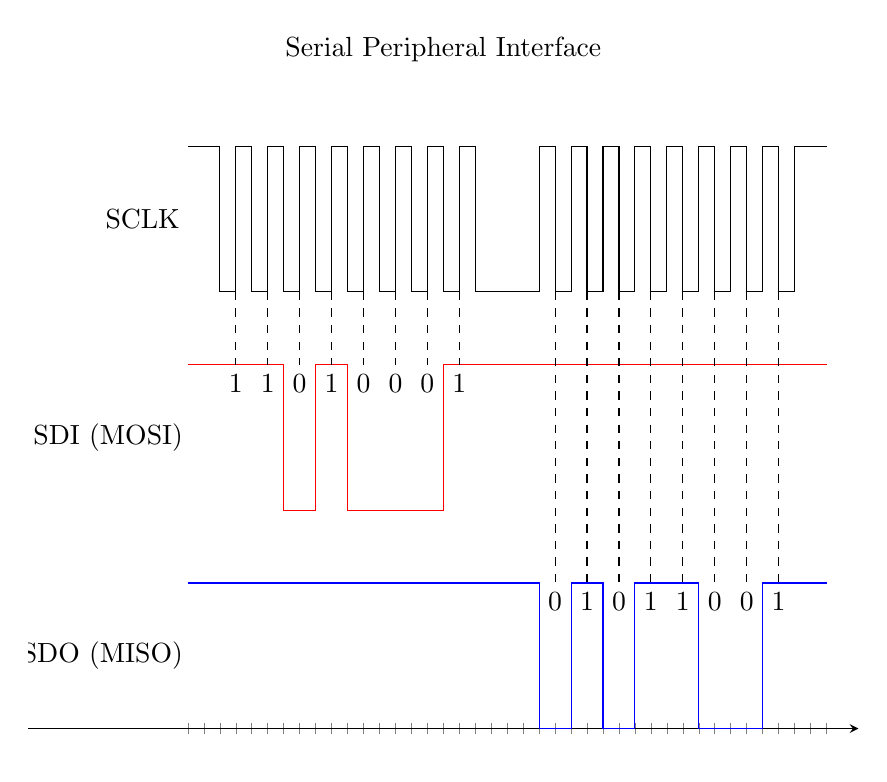
\begin{tikzpicture}
    \begin{axis}[
        width=\textwidth,
        axis x line=middle,
        axis y line=none,
        xmajorgrids=false,
        grid style=dashed,
        xtick={0,10,...,400},
        xmin=-100,
        xmax=420,
        samples=1000,
        title=Serial Peripheral Interface,
        xticklabels=\empty,
    ]
    % SCK
    \addplot[black] coordinates
    {(0,8) (20,8) (20,6) (30,6) (30,8) (40,8) (40,6) (50,6) (50,8) (60,8) (60,6) (70,6) (70,8)
    (80,8) (80,6) (90,6) (90,8) (100,8) (100,6) (110,6) (110,8) (120,8) (120,6) (130,6) (130,8) 
    (140,8) (140,6) (150,6) (150,8) (160,8) (160,6) (170,6) (170,8) (180,8) (180,6) (220,6) 
    (220,8) (230,8) (230,6) (240,6) (240,8) (250,8) (250,6) (260,6) (260,8) (270,8) (270,6)
    (280,6) (280,8) (290,8) (290,6) (300,6) (300,8) (310,8) (310,6) (320,6) (320,8) (330,8) (330,6) 
    (340,6) (340,8) (350,8) (350,6) (360,6) (360,8) (370,8) (370,6) (380,6) (380,8) (400,8)};
    
    % SDI (MOSI)
    \addplot[red] coordinates
    {(0,5) (60,5) (60,3) (80,3) (80,5) (100,5) (100,3) (160,3) (160,5) (400,5)};
    
    % SDO (MISO)
    \addplot[blue] coordinates
    {(0,2) (220,2) (220,0) (240,0) (240,2) (260,2) (260,0) (280,0) (280,2) (320,2) (320,0) (360,0)
    (360,2) (400,2)};

    % Draw Dashed Lines
    \draw[dashed] (axis cs:30,6) -- (axis cs:30,5) node[below] {1}
        (axis cs:50,6) -- (axis cs:50,5) node[below] {1}
        (axis cs:70,6) -- (axis cs:70,5) node[below] {0}
        (axis cs:90,6) -- (axis cs:90,5) node[below] {1}
        (axis cs:110,6) -- (axis cs:110,5) node[below] {0}
        (axis cs:130,6) -- (axis cs:130,5) node[below] {0}
        (axis cs:150,6) -- (axis cs:150,5) node[below] {0}
        (axis cs:170,6) -- (axis cs:170,5) node[below] {1};

    \draw[dashed] (axis cs:230,6) -- (axis cs:230,2) node[below] {0}
    (axis cs:250,6) -- (axis cs:250,2) node[below] {1}
    (axis cs:270,6) -- (axis cs:270,2) node[below] {0}
    (axis cs:290,6) -- (axis cs:290,2) node[below] {1}
    (axis cs:310,6) -- (axis cs:310,2) node[below] {1}
    (axis cs:330,6) -- (axis cs:330,2) node[below] {0}
    (axis cs:350,6) -- (axis cs:350,2) node[below] {0}
    (axis cs:370,6) -- (axis cs:370,2) node[below] {1};

    % Draw SDI, SCK etc.
    \draw (axis cs:1,7) node[left] {SCLK}
        (axis cs:3,4) node[left] {SDI (MOSI)}
        (axis cs:3,1) node[left] {SDO (MISO)};

    \end{axis}
    \end{tikzpicture}
\end{center}
\caption{SPI Transmission Waveform}
\label{fig:spi-wave}
\end{figure}
